

\section{Introduction}
{\co Comme le souligne Corliss \cite{Corliss1991b}, la DA est une technique introduite vers 1962 avec le mode direct mais n'a pas r\'eussi \`a s'imposer.
 Ce n'est que plus tard, en 1982, grâce \`a l'am\'elioration des techniques de programmations et l'introduction du mode inverse que la DA a
 connu plus de succ\`es.
Griewank est \`a l'origine de grands progr\`es et il s'en ait suivi une forte augmentation du nombre d'outils, de techniques et d'applications 
de la diff\'erentiation automatique. 
L'implantation de la DA se divise en deux formes : la surcharge des op\'erateurs et la transformation du code.
La surcharge des op\'erateurs consitent \`a \'etandre la s\'emantique des op\'erations, c'est-\`a-dire que chaque variable est surcharg\'ee
par sa d\'eriv\'ee et les op\'erations s'op\`erent ces les deux quantit\'es. }
La tranformation de code, ne fait que retourner le code de la d\'eriv\'ees. Le code est analys\'e puis transformer, en fait les lignes 
correspondant au calcul de la diff\'erenti\'ee sont rajout\'ees. Ce code est parfois \'ecrit \`a la main mais la DA a suffisamment fait de progr\`es pour g\'en\'erer un code en quelques minutes (pour les gros programmes) et 
d'une qualit\'e comparable d'apr\`es l'article \cite{diffautoopa}.

 Nous verrons ainsi quelles sont les points forts et faibles de ces deux
proc\'ed\'es.



% --------------------- \`a am\'eliorer -------------------------------
% Il existe deux formes diff\'erentes de DA. Soit par transformation de code, qui analyse le code original pour produire le 
% code de la diff\'erenti\'ee ; le code adjoint. Il est parfois \'ecrit
% \`a la main mais la DA a suffisamment fait de progr\`es pour g\'en\'erer un code en quelques minutes (pour les gros programmes) et 
% d'une qualit\'e comparable d'apr\`es l'article \cite{diffautoopa}.
% Soit la surcharge des op\'erateurs qui consiste \`a sp\'ecifier les calculs de 
% d\'erivation associ\'es \`a chaque op\'eration effectu\'ee.
% --------------------- \`a am\'eliorer -------------------------------


% explication de la diff\'erentiatation automatique : diff\'erence avec la
% diff\'erentiation symbolique et par diff\'erences finies
%

Ainsi, comme indiqu\'e dans \cite{differentiaauto}, le but de la DA est de calculer la d\'eriv\'ee d'une fonction sp\'ecifi\'ee par
un programme, un algorithme. Cette m\'ethode de calcul s'oppose \`a deux autres
bien connues : la diff\'erentiation symbolique et la diff\'erentiation par
diff\'erences finies. La premi\`ere, que l'on peut retrouver dans {\it Maple}, 
utilise l'expression de la fonction pour d\'eterminer sa d\'eriv\'ee.
Cette technique est tr\`es vite limit\'ee d'une part lorsque l'on a des
expressions un peu complexes et d'autre part parce qu'il faut l'expression de la
fonction. \\
Par exemple sur {\it Maple}, si on veut obtenir :
\[\frac{\partial^3((x^2+y^2)*(\ln(x)-\ln(y)))}{\partial y \partial^2x}\]
\verb!diff((x^2+y^2)*(ln(x)-ln(y)), y,x$2);!\\
$\rightarrow$ $-\frac{2y}{x^2}-\frac{2}{y}$
\\
%

{\co
Griewank illustre un exemple de diff\'erentiation symbolique dans \cite{Iri89onautomatic}, avec le logiciel {\it Macsyma}. La fonction
qui permet de calculer l'energie d'Helmholtz est fournie au logiciel. Le r\'esultat correspond \`a la figure \ref{fig:macsyma}. 
En plus du fait que le code g\'en\'er\'e est difficilement comprehensible pour un être humain, le code a du être modifi\'e \`a cause 
du maximum de 19 lignes cons\'ecutives en Fortran. Ainsi, il est extrêment difficile de pouvoir maintenir une telle structure de code.
}

\begin{figure}
\caption{Code produit par diff\'erentiation symbolique \`a partir du logiciel {\it Macsyma}}
\begin{center}
\fbox{
\begin{minipage}[c]{0.7\textwidth}
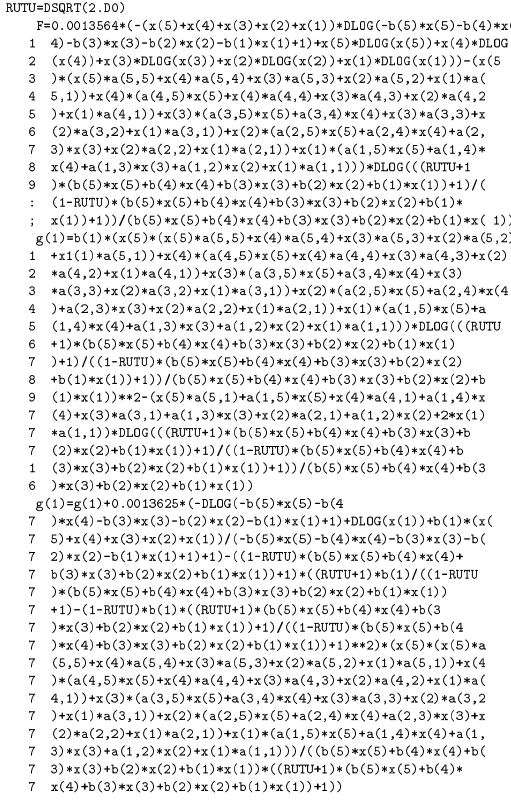
\includegraphics[scale=0.7]{figures/macsyma.png}
\end{minipage}
}
\end{center}
\label{fig:macsyma}
\end{figure}


% 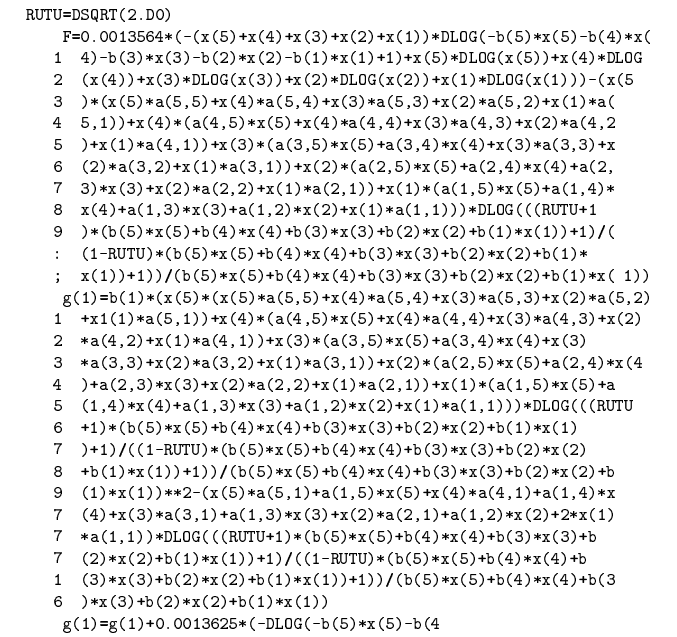
\includegraphics[scale=0.5]{figures/macsyma1.png}\\
% 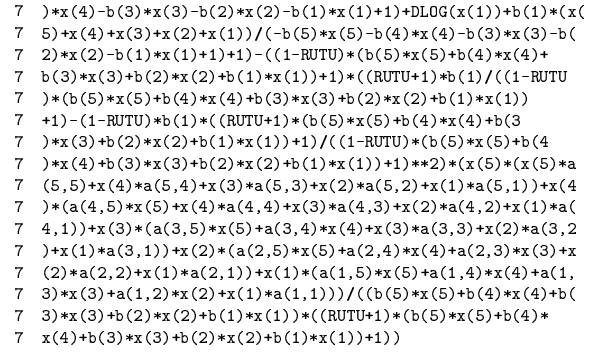
\includegraphics[scale=0.5]{figures/macsyma2.png}\\

La  plupart du temps, il faut diff\'erentier un code constitu\'e de
boucles et de conditions qui est difficilement exprimable par une expression
math\'ematique.
 La diff\'erentiation num\'erique ou par diff\'erences finies
s'appuie sur l'expression th\'eorique de la d\'eriv\'ee: 
$$\lim_{h\rightarrow 0}\frac{f(x+h)-f(x)}{h}$$
Dans le cas \`a plusieurs dimensions:
$$\lim_{\varepsilon \rightarrow 0}\frac{P(X+\varepsilon \cdot dX)-P(X)}{\varepsilon} =
 \nabla P(X)\cdot dX$$
Cependant, il s'agit d'un probl\`eme hasardeux \`a cause de la
discr\'etisation impos\'ee par ordinateur. $h$ doit être choisi dans l'ordre de
 grandeur de la racine de la pr\'ecision machine : si $h$ est trop proche de $0$ la
diff\'erence va être mal approch\'ee ; l'\'ecart entre $f(x+h)$ et $f(x)$
 \'etant trop faible et si $h$ est trop grand, on s'\'eloigne de la v\'eritable
valeur de la d\'eriv\'ee. Ainsi, nous allons voir que la diff\'erentiation
automatique pallie \`a ces deux inconv\'enients majeurs. \\






\section{Principes de la diff\'erentiation automatique}
\label{sec:da}

{\co Contrairement \`a la diff\'erentiation symbolique, l'objectif de la diff\'erentiation automatique n'est pas de concevoir l'expression de la d\'eriv\'ee mais uniquement
le programme qui la calcule.}
La DA calcule la d\'eriv\'ee de mani\`ere analytique, c'est-\`a-dire qu'elle obtient le calcul exact de la d\'eriv\'ee. Ainsi, il n'y a pas d'erreurs
d'approximations. \`A chaque fois qu'appara\^it une variable dans le programme source,
le programme diff\'erenti\'e va calculer une variable additionnelle de la même forme : sa diff\'erenti\'ee.
Il est \`a noter que la DA ne vise pas \`a fournir l'expression math\'ematique de la d\'eriv\'ee, puisqu'elle ne fournit que du
code permettant son \'evaluation.
Il existe deux mani\`eres d'utiliser la DA, soit le code est transform\'e pour obtenir un nouveau programme qui
calculera directement la diff\'erenti\'ee, soit par surcharge des op\'erateurs. Nous allons d\'ecrire en d\'etail ces diff\'erentes approches.
Pour la deuxi\`eme approche, il s'agit d'ajouter aux fonctions de base (l'addition, cos, log) les op\'erations de d\'erivations.

Par exemple, en prenant {\tt x}, {\tt y}, {\tt z} comme variables et {\tt V} comme vecteur,
lors de l'instruction :\\
$${\tt x= y*V(10)+z}$$\\
le programme diff\'erenti\'e va  calculer :
$$\dot{\tt x}= \dot{\tt y}*{\tt V(10)} + {\tt y}*\dot{\tt V}{\tt(10)}+\dot{\tt z} $$
en utilisant les r\`egles de d\'erivations usuelles sur les fonctions. Il n'y a plus
d'approximations, c'est un calcul exact. 
Le principe est de consid\'erer que chaque programme peut s'\'ecrire comme une s\'equence
d'instructions.
$$I_1;I_2;...;I_{p-1};I_{p}$$
Cette suite peut être identifi\'ee comme une composition de fonctions 
$$f=f_p\circ f_{p-1} \circ \cdots \circ f_1$$
par la r\`egle de d\'erivation sur la composition~(\ref{annexe:A}) on obtient :\\

\begin{align*}
f'(X) = & (f'_p\circ f_{p-1} \circ f_{p-2} \circ ... \circ f_1(X))\\
& . (f'_{p-1} \circ f_{p-2} \circ ... \circ f_1(X))\\
& \cdots\\
& . f'_1(X)\\
= & f'_p(W_{p-1}) . f'_{p-1}(W_{p-2}) . \cdots .f'_1(W_0).\\
\end{align*}
En notant $W_0=X$ et $W_k=f_k(W_{k-1})$.
%
Comme plusieurs donn\'ees sont trait\'ees, tous les $f'_k$ sont des matrices Jacobiennes de 
taille relativement grande dans un cas g\'en\'eral. Calculer la diff\'erenti\'ee revient \`a calculer
les multiplications de ces matrices. Cependant, il n'est pas possible de calculer ce produit avec un co\^ut 
raisonnable. Par exemple, avec dix variables, si on effectue une quinzaine d'instructions
cela revient \`a faire de l'ordre de $10^4$ op\'erations. La complexit\'e est exponentielle. Dans la plupart
des cas, l'application qui utilise $\nabla f(X)$  n'a en r\'ealit\'e que besoin d'une direction de la jacobienne :
 $\nabla f(X).\dot{X}$ pour une certain vecteur $\dot{X}$.
Nous allons voir les deux modes de diff\'erentiation, le mode tangent et le mode inverse. Dans le premier mode, 
les calculs de la fonctions se propagent parall\`element aux d\'eriv\'ees tandis que dans le mode inverse, le calcul
s'effectue \`a rebours en partant de la fin du code.







    \subsection{Mode tangent ou mode direct}

\label{chap2:tangent}
Dans notre cas, comme par exemple pour la direction de Chebychev, nous avons besoin de calculer $\nabla^3f(x)\cdot u\cdot v$ et non $\nabla^3f(x)$.
 En prenant cela en compte, le calcul va être largement simplifi\'e. \`A l'ordre un : $\dot{Y}=f'(X).\dot{X}$
$$\dot{Y}=f'_p(W_{p-1}) . f'_{p-1}(W_{p-2}) . \cdots .f'_1(W_0).\dot{X}.$$\\
Pour profiter de la multiplication avec le vecteur, le calcul va se faire de droite \`a gauche afin d'\'eviter d'avoir des multiplications de 
Matrice$\times$Matrice (correspond au mode multi-directionnel pour Tapenande) mais plut\^ot Matrice$\times$Vecteur. De plus, de cette mani\`ere, les appels aux $W_i$ vont
se faire dans l'ordre, donc en même temps qu'ils seront calcul\'es. Cette m\'ethode donne une combinaison lin\'eaire des 
colonnes de la matrice Jacobienne.
Voici un exemple illustr\'e pour la fonction $f(x_1,x_2)=(x_1-cos(x_2))^2$. Dans le Graphe Acyclique Orient\'e \ref{fig:gao}, le 
gradient de chaque quantit\'e en partant des feuilles va être propag\'e.


\begin{figure}
\caption{GAO : $f(x_1,x_2)=(x_1-cos(x_2))^2$ pour \'evaluer la fonction, le parcours se fait 
\`a partir des feuilles de l'arbre jusqu'\`a la racine.}
\begin{center}
\fbox{
\begin{minipage}[c]{0.45\textwidth}
\beginpgfgraphicnamed{figures/figure_14}
\endpgfgraphicnamed
\end{minipage}
}
\end{center}
\label{fig:gao}
\end{figure}




% \floatstyle{ruled}
% \newfloat{Program}{tbp}{lop}[section]
% \begin{Program}
% \begin{verbatim}
% . . . program text . . .
% \end{verbatim}
% \caption{. . . caption . . . }
% \end{Program}








\begin{figure}
\caption{GAO : mode tangent, il suit le même parcours que celui de l'\'evaluation}
\begin{center}
\fbox{
\begin{minipage}[c]{0.6\textwidth}
\beginpgfgraphicnamed{figures/figure_11}
\endpgfgraphicnamed
\end{minipage}
}
\end{center}
\label{fig:modetangent}
\end{figure}



\vspace{1cm}
\begin{tabular}{|l|c|l|c|c|}
  \hline
  $y$ & Valeurs de $y$ & $\dot{y}$ & Valeurs de $\dot{y}$ & Valeurs vectorielles
\\
  \hline
  $y_1$ &  $x_1$ &  $\dot{y_1}$ & $\dot{x_1}$ & [$1$ \ $0$] \\
  $y_2$ & $x_2$ & $\dot{y_2}$ & $\dot{x_2}$ & [$0$ \ $1$] \\
  $y_3$ & $cos(y_2)$ & $\dot{y_3}$ & $-\dot{y_2}sin(y_2)$ & -[$0$ \ $sin(x_2)$]
\\
  $y_4$ & $y_1-y_3$ & $\dot{y_4}$ & $\dot{y_1}-\dot{y_3}$ & [$1$ \ $sin(x_2)$]
\\
  $y_5$ & $y_4^2$ &  $\dot{y_5}$ & $2\dot{y_4}y_4$ & $2$[$x_1-cos(x_2)$ \
$(x_1-cos(x_2))sin(x_2)$]\\
  
  \hline
\end{tabular}



\vspace{1cm}

Le programme g\'en\'er\'e par la DA \'evalue simultan\'ement la fonction et le gradient. Le nombre de lignes obtenu
est environ deux fois celui du programme d'origine puisque chaque affectation est accompagn\'ee du calcul du
gradient. En g\'en\'eral, comme c'est expliqu\'e dans \cite{Iri89onautomatic}, le mode tangent multiplie le nombre
 d'op\'erations arithm\'etiques de $n$. Chaque quantit\'e 
$x_i$ est pr\'ec\'ed\'ee du calcul de $\nabla x_i$ de taille $n$. Dans l'exemple, on peut observer que les quantit\'es propag\'ees ont 
une dimension \'equivalente au nombre de composante de l'argument. Ainsi, le coût dû au calcul du gradient est de l'ordre de 
$n$ fois le co\^ut de l'\'evaluation de la fonction.
\vspace{0.51cm}



% \end{figure}

% 

    \subsection{Mode inverse}
{\co Comme nous venons de le voir, le mode tangent propage un vecteur de la taille du gradient dans le graphe, par cons\'equent, le coût 
est proportionnel \`a $n\#(f)$. En revanche, le mode inverse ne va que propager un scalaire dans le graphe mais le parcours va se faire dans le 
sens inverse \`a celui de l'\'evaluation. C'est parce que les calculs ne se font que sur un scalaire que le coût du gradient est proportionnel
 au coût de l'\'evaluation de la fonction. 
Ainsi, il va être pr\'ef\'erable de choisir le mode inverse au mode tangent.}

Le mode inverse va nous permettre d'obtenir une ligne de la Jacobienne c'est-\`a-dire un gradient par rapport \`a 
une composante $k$.
$$\overline{X}=f'^T(X).\overline{Y}$$ 
\begin{equation}\overline{X}=f_{1}^{'T}(W_{0}) . f_{2}^{'T}(W_{1}) . \cdots .f_p^{'T}(W_{p-1}) . \overline{Y}
\label{eq:inv}
\end{equation}
L'id\'ee sous-jacente est l'utilisation des quantit\'es adjointes :

$$y_i^*= \frac{\partial f}{\partial y_i} $$
% $$y_j^*= \sum \frac{\partial f}{\partial y_j}y_i^*$$
$$\bar{y_j}= \sum_{i \in I_j} \frac{\partial f}{\partial y_j}\bar{y_i}$$
% $$\text{ o\`u tous les }\bar{y_i}\text{ sont des quantit\'es scalaires }$$
o\`u tous les $\bar{y_i}$ sont des quantit\'es scalaires
 $$I_j=\{i | y_j \text{ intervenant dans } y_i\}.$$


Le parcours du GAO se fait en profondeur, de la racine jusqu'aux feuilles. Contrairement au mode tangent,
comme les quantit\'es propag\'ees sont des scalaires, qu'une seule \'equation n'est impliqu\'ee \`a chaque n\oe ud,
 au lieu d'en avoir $n$, la dimension. Comme l'indique la figure \ref{fig:modeinverse}, les quantit\'es $\bar{y_i}$ se
propagent \`a rebours, dans le sens inverse des quantit\'es $\dot{y_i}$. C'est le fait
que le calcul se propage sur l'ensemble des feuilles qui va permettre de reconstruire le gradient de dimension $n$, chaque feuille
correspondant \`a une composante.
Commençons par observer ce mode sur notre exemple. Cette fois-ci, le parcours n'est plus le même que 
l'\'evaluation de la fonction.


\begin{figure}
\caption{GAO : mode inverse, cette fois-ci, l'arbre est parcouru depuis la racine.}
\begin{center}
\fbox{
\begin{minipage}[c]{0.75\textwidth}
\beginpgfgraphicnamed{figures/figure_12}
\endpgfgraphicnamed
\end{minipage}
}
\end{center}
\label{fig:modeinverse}
\end{figure}


\vspace{1cm}
\begin{tabular}{|l|c|}
  \hline
  $y$ & Valeurs de $y$ \\
  \hline
  $y_1$ & $x_1$ \\
  $y_2$ & $x_2$ \\
  $y_3$ & $cos(y_2)$ \\
  $y_4$ & $y_1-y_3$ \\
  $y_5$ & $y_4^2$ \\
  \hline
\end{tabular}
\hspace{1cm}
\begin{tabular}{|l|c|c|}
  \hline
 $\bar{y}$ & Valeurs de $\bar{y}$ & Valeurs \\
  \hline
 $\bar{y_5}$ & $1$ & $1$ \\
 $\bar{y_4}$ & $2y_4$ & $2(x_1-cos(x_2))$ \\
 $\bar{y_3}$ & $-\bar{y_4}$ & $2(cos(x_2)-x_1)$ \\
 $\bar{y_2}$ & $-\bar{y_3}sin(x_2)$ & $2(x_1-cos(x_2))sin(x_2)$ \\
 $\bar{y_1}$ & $\bar{y_4}$ & $2(x_1-cos(x_2))$ \\
  \hline
\end{tabular}\\

\noindent
%D'apr\`es Griewank \ref{Iri89onautomatic}, {\bf le co\^ut d'\'evaluation du gradient n\'ecessite jamais plus cinq fois le co\^ut de l'\'evaluation de la fonction}.
Dans l'\'equation \ref{eq:inv}, l'op\'eration doit se faire encore de droite \`a gauche pour que le calcul soit efficace. Malheureusement, cette fois-ci,
nous n'avons pas les appels aux $W_i$ dans le même ordre qu'ils sont calcul\'es; cela vient du fait que le parcours
n'est plus dans le même sens. Dans l'exemple, \`a la deuxi\`eme \'etape, la 
quantit\'e $y_4$ est n\'ecessaire, elle fait intervenir $y_1$ et $y_2$ alors que ces \'etats n'ont pas encore \'et\'e parcourus.
Ainsi, il existe deux strat\'egies pour obtenir les $W_i$. Soit on recalcule toutes les quantit\'es, soit on les m\'emorise toutes.




    \subsection{Strat\'egies de la DA pour le mode inverse}
% point noir stockage
% point blanc
% 
% $\overline{I_k} \rightarrow \overline{W_{k-1}}=f_k^{'T}(W_{k-1}).\overline{W_k}$
% 
\label{subsection:strategies}
 \paragraph{Recompute-All}
%  \\
Pour chaque terme $W_p=f_k(W_{p-1})$, on recalcule l'ensemble de la suite $W_i$ \`a chaque fois. L'op\'eration $W_1 =f'(X)$ va être effectu\'ee $p$ fois.
 Cette m\'ethode demande plus de temps d'ex\'ecution puisque les termes ne sont pas m\'emoris\'es, les mêmes 
calculs sont effectu\'es plusieurs fois. {\co Sur les figures commençant \`a \ref{fig:ra} jusqu'\`a \ref{fig:checkpointsa}}, les points noirs repr\'esentent le stockage de $W_k$ sur la pile
d'ex\'ecution et les points blancs repr\'esentent un d\'epilement.


% \vspace{1cm}
\begin{figure}
\caption{Strat\'egie RA : pour chaque quantit\'e \`a calculer, on reparcours le graphe pour faire un pas dans l'algorithme inverse. Prend moins de place mais
plus de temps.}
\fbox{
\begin{minipage}[c]{0.9\textwidth}
\beginpgfgraphicnamed{figures/figure_3}
\endpgfgraphicnamed
\end{minipage}
}
\label{fig:ra}
\end{figure}
% \vspace{1cm}


 \paragraph{Store-All}
Cette fois-ci, tous les termes vont être calcul\'es et enregistr\'es une seule fois. Il s'agit d'une
m\'ethode qui n\'ecessite plus de m\'emoire. Le co\^ut en m\'emoire est lin\'eaire par rapport \`a $p$.


% \vspace{1cm}
\begin{figure}
\caption{Strat\'egie SA : le graphe des \'evaluations est parcouru une seule fois pour toutes les m\'emoriser, l'algorithme inverse n'aura plus qu'\`a d\'epiler. Prend
moins de temps mais plus de capacit\'e de stockage.}
\begin{center}


\fbox{
\begin{minipage}[c]{0.9\textwidth}
\beginpgfgraphicnamed{figures/figure_4}
\endpgfgraphicnamed
\end{minipage}
}

% \beginpgfgraphicnamed{figures/figure_4}
% \endpgfgraphicnamed

\end{center}
\label{fig:sa}
\end{figure}
% \vspace{1cm}



Dans les deux cas, si le probl\`eme a une dimension trop grande, ni la strat\'egie RA, ni la SA ne pourra être
efficace. Une m\'ethode alternative appara\^it comme un bon compromis : le {\it Checkpointing}.
L'id\'ee est de d\'ecomposer le programme en plusieurs parties, si possible imbriqu\'ees et d'effectuer une sauvegarde, un {\it snapshot},
des quantit\'es entre chaque. Encore peu de travail a \'et\'e effectu\'e sur la comparaison de l'emplacement de ces {\it Checkpoints} et cela
reste une probl\`eme ouvert. Il n'y a pour l'instant pas d'emplacement optimal connu pour un algorithme quelconque. N\'eanmoins, 
ils seront \'evidemment plac\'es \`a l'ext\'erieur des sous-routines ou des boucles. \`A partir des ces 
sauvegardes on peut soit appliquer la m\'ethode RA sur la sous partie du code comme l'illustre la figure \ref{fig:checkpointra}, soit
la m\'ethode SA \ref{fig:checkpointsa}. C'est la deuxi\`eme qui a \'et\'e retenue par {\it Tapenade} car la taille de la pile est dans ce cas 
raisonnable et les ex\'ecutions d'empilement et de d\'epilement sont rapides.


\begin{figure}
\caption{Checkpoint RA - on effectue des sauvegardes \`a certains
n\oe uds du GAO et entre chacun de ces n\oe uds on adopte une strat\'egie de tout recalculer.}
\begin{center}
\fbox{
\begin{minipage}[c]{0.9\textwidth}
\beginpgfgraphicnamed{figures/figure_5}
\endpgfgraphicnamed
\end{minipage}
}
\end{center}
% \beginpgfgraphicnamed{figures/figure_5}
% \endpgfgraphicnamed
\label{fig:checkpointra}
\end{figure}
% \vspace{1cm}

\begin{figure}
\caption{Checkpoint SA - l\`a aussi, on sauvegarde les donn\'ees \`a certains n\oe uds mais entre
chaque on utilise une strat\'egie de tout m\'emoriser.}


\fbox{
\begin{minipage}[c]{0.9\textwidth}
\beginpgfgraphicnamed{figures/figure_6}
\endpgfgraphicnamed
\end{minipage}
}



% \beginpgfgraphicnamed{figures/figure_6}
% \endpgfgraphicnamed
\label{fig:checkpointsa}
\end{figure}
\vspace{1cm}




\section{Implantation de la DA}

Deux possibilit\'es s'offrent, soit la surcharge des op\'erateurs, plus flexible, soit la transformation du code.
Dans le premier cas, les op\'erateurs vont être transform\'es pour ajouter les op\'erations de d\'erivation alors que dans
la transformation du code, on ne fait qu'analyser et modifier le code texte qui permet les calculs de la fonction.



\subsection{La surcharge des op\'erateurs}
{\co
Comme l'a fait Karczmarczuk dans l'article \cite{paresseuse}, il est possible de programmer la diff\'erentiation automatique 
par surcharge des op\'erateurs avec un langage fonctionnel. Voir l'annexe \ref{annexe:C}. Malheureusement, les structures de donn\'ees 
sont tr\`es rapidement lourdes \`a g\'erer, surtout qu'il s'agit de listes paresseuses infinies. Bien qu'il s'av\`ere être un outil simple \`a 
manipuler, il n'est pas possible d'obtenir une efficacit\'e acceptable. D'autre part, un outil de surcharge des op\'erateurs \`a \'et\'e effectu\'e
pour {\it Scilab} nomm\'e sciad par Benoit Hamelin. Cependant, il souffre d'un grand overhead et les temps d'ex\'ecution sont long lorsque
la dimension est plus grande que $5$. D'autre part, cette approche consiste \`a faire l'acquisition du graphe en surchargeant les op\'erateurs usuels
et les fonctions \'el\'ementaires, cependant il n'est pas possible de surcharger les structures de contrôle comme les comparaisons et les boucles.
Par cons\'equent, si une condition vient \`a changer, il faut proc\'eder \`a une nouvelle aquisition du graphe alors que dans le cas par 
transformation de code, l'int\'egralit\'e du programme est transform\'e, donc cette difficult\'e n'apparaît pas.}



\subsection{La transformation du code}
Ce proc\'ed\'e n'utilise que le code de la fonction pour g\'en\'erer celui de la d\'eriv\'ee.
Au lieu de surcharger les op\'erateurs, le code est analys\'e pour d\'etecter les variables d\'ependantes.
Ensuite, par un proc\'ed\'e analytique, il applique la d\'erivation sur les op\'erations usuelles; 
{\tt sin(x)} est transform\'ee en {\tt cos(x)*xd} o\`u {\tt xd=}$\dot x$ et il rajoute cette ligne
juste avant.

 Si on reprend le mode tangent sur notre exemple : comme variable de sortie, on a {\tt f} et 
comme variable d'entr\'ee {\tt x}. {\co En Fortran, l'exposant se note {\tt **}.} \\


{\tt
\begin{tabular}{|l|l|}
  \hline
  Code original & Mode tangent \\
  SUBROUTINE F(x, f) & SUBROUTINE F\_d(x, xd, f, fd) \\
  \hline
			& fd = xd(1) + xd(2)*SIN(x(2)) \\
    f=x(1)-COS(x(2))	& f = x(1) - COS(x(2))\\
			& fd = 2*f*fd\\
    f=f**2    		& f = f**2\\  
  \hline
\end{tabular}
}\\

Ainsi, dans le mode tangent, la valeur {\tt fd} renvoie $\nabla F(x).xd$, en {\it Scilab} \\ 
{\tt derivative(F,x)*xd}.
Ce code, nomm\'e code adjoint, reste tr\`es proche du code d'origine et est imp\'eratif. {\co Il b\'en\'eficiera ainsi d'une ex\'ecution 
efficace.

Le tableau ci-dessous donne \`a gauche le code du programme de notre fonction et \`a droite il s'agit de r\'esultat retourn\'e par 
l'outil que nous utiliserons plus tard. L'outil g\'en\`ere des noms d'incr\'ement \'evitant des conflits d'o\`u {\tt ii1}.} \\



{\tt
\begin{tabular}{|l|l|}
  \hline
  Code original & Mode reverse \\
  SUBROUTINE F(x, f) & SUBROUTINE F\_b(x, xb, f, fb) \\
  \hline


     f=x(1)-COS(x(2))   &  f = x(1) - COS(x(2)) \\
     f=f**2	          &  fb = 2*f*fb \\
			  &  DO ii1=1,2 \\
			  &    xb(ii1) = 0.D0 \\
			  &  ENDDO \\
			  &  xb(1) = fb \\
			  &  xb(2) = SIN(x(2))*fb \\
			  &  fb = 0.D0 \\
			  &  END \\
  \hline
\end{tabular}
} \\
\vspace{0.5cm}
\\{\tt xb} renvoie la valeur du gradient, en {\it Scilab}, cela correspond \`a la ligne de commande\\ {\tt ---> xb=derivative(F,x)*fb}.



\subsection{Discussion}

La surcharge des op\'erateurs est plus souple et plus simple \`a utiliser. Il suffit en g\'en\'eral d'enrichir le type de donn\'ees pour effectuer
la diff\'erentiation sur ce nouveau type. La transformation de code source se fait en amont et utilise 
des concepts issus de la compilation en arbre de syntaxe. 
Maintenant que nous venons de voir les principes de fonctionnement, il a fallu
choisir un outil de diff\'erentiation automatique permettant d'implanter 
efficacement les op\'erations : $\nabla f$, $\nabla^2 f\cdot v$, $\nabla^2 f$, $\nabla^3 f\cdot u\cdot v$, $\nabla^3 f\cdot u$, 
$\nabla^4 f\cdot u\cdot v\cdot w$. Malgr\'e le fait 
qu'il existe actuellement plusieurs outils de DA, le choix n'est pas \'evident car pour une 
impl\'ementation efficace, il est pr\'ef\'erable d'utiliser un outil par transformation de code et 
le fait d'obtenir des d\'eriv\'ees sup\'erieures est en g\'en\'eral un point fort de la surcharge des 
op\'erateurs.
De plus, nous avons dû choisir une banque de tests ad\'equate \`a notre outil et qui repr\'esente 
suffisamment de cas de figure afin de tester correctement les algorithmes. Nous allons ainsi pr\'esenter
les temps d'ex\'ecution pour l'ensemble des op\'erations; gradient, hessien, etc...







